% =====================================================================
%  Differentiable DTL reconciliation (gpurec) — paper source
%  Compiles with: latexmk -pdf gpurec_paper.tex
% =====================================================================
\documentclass[11pt]{article}

\usepackage[utf8]{inputenc}
\usepackage[T1]{fontenc}
\usepackage{amsmath,amssymb,amsthm}
\usepackage{graphicx}
\graphicspath{{figures/}}
\usepackage{booktabs}
\usepackage{xcolor}
\usepackage[margin=1in]{geometry}
\usepackage{microtype}
\usepackage[round,authoryear]{natbib}
\usepackage[colorlinks=true,allcolors=blue]{hyperref}
\usepackage{enumitem}
\usepackage{xspace}

% ---- tool name (change in one place) -------------------------------
\newcommand{\toolname}{\textsc{gpurec}\xspace}

% ---- highlighted callout box ---------------------------------------
% Use \begin{expbox}{short title} ... \end{expbox} for a boxed summary.
\newenvironment{expbox}[1]{%
  \par\smallskip\noindent
  \begin{center}\begin{minipage}{0.96\linewidth}\small
  \rule{\linewidth}{0.8pt}\par
  \textbf{#1}\par
}{%
  \par\rule{\linewidth}{0.8pt}
  \end{minipage}\end{center}\smallskip
}
% inline status note (for items still in progress)
\newcommand{\status}[1]{{\color{gray!50!black}\emph{#1}}}
\newcommand{\TODO}[1]{{\color{red!70!black}\textbf{[TODO: #1]}}}

% ---- math shortcuts ------------------------------------------------
\newcommand{\bdelta}{\delta}
\newcommand{\btau}{\tau}
\newcommand{\blambda}{\lambda}
\newcommand{\NLL}{\mathcal{L}}
\newcommand{\Hess}{\mathbf{H}}
\newcommand{\Fish}{\mathbf{I}}
\newcommand{\grad}{\mathbf{g}}
\newcommand{\Real}{\mathbb{R}}

\title{\textbf{Differentiable DTL Reconciliation:\\
Certified Optima, Identifiability Diagnostics, and\\
Transfer-Recipient Heterogeneity in Archaeal Gene Families}}

\author{Enzo Marsot}
\date{\today}

\begin{document}
\maketitle

% =====================================================================
\begin{abstract}
\noindent
Reconciling gene trees with a species tree under a model of gene
\emph{duplication, transfer, and loss} (DTL) is central to comparative
genomics. Existing reconciliation software --- including the state-of-the-art
\textsc{AleRax} --- treats the amalgamated likelihood as a fixed, hand-%
differentiated black box, optimized by first-order methods on the CPU. We
re-implement the \textsc{UndatedDTL} reconciliation likelihood as a fully
\emph{differentiable} GPU program, exposed through a \textsc{PyTorch} interface.
Our central claim is methodological: \emph{differentiable reconciliation is an
enabling computational paradigm} --- analytic gradients, Hessian--vector products,
the observed-information matrix, uncertainty quantification, custom priors, and
model extensions all follow from it, essentially for free. Concretely it yields
(i) \emph{second-order} inference --- certified \emph{local} optimality via the
Hessian spectrum, and the observed-information matrix for parameter uncertainty and
a duplication--loss non-identifiability diagnosis; (ii) \emph{per-recipient transfer
weights} that relax the uniform-recipient assumption (a feature listed as future
work for \textsc{AleRax}) together with a likelihood test of it; and (iii)
\emph{arbitrary user-defined penalties}, demonstrated by cross-validating a
tree-smoothing prior for species-wise rates on \textsc{Hogenom} --- all made
practical at genome scale by GPU throughput that, as a by-product, delivers
order-of-magnitude faster genewise rate estimation. On the empirical
\textsc{Hogenom-Core} and archaeal datasets, \toolname localises the
duplication--loss non-identifiability and cross-validates the tree-smoothing prior
that mitigates it, certifies a bound-constrained optimum of the $357$-parameter
archaeal species-wise rate fit, and finds per-recipient transfer heterogeneity
decisively favoured on the archaeal data --- in-sample $\Delta\mathrm{AIC}\approx
13{,}900$ for the $118$ added recipient weights, and out-of-sample the weights lower
held-out NLL by $\approx\!1{,}360$ nats ($1.25$ per held-out family, nearly the
in-sample gain, so the heterogeneity generalizes); the underlying throughput fits
all $10{,}869$
per-family rate sets in $13$ minutes on a single \textsc{RTX 4090}
($\sim\!23\times$ faster than \textsc{AleRax} on $24$ CPU cores, at marginally
higher likelihood), which is what makes the cross-validation and diagnostics above
feasible. Differentiable reconciliation thus turns the DTL
likelihood from a point-estimation black box into a statistically interrogable
model --- one that certifies its optima, quantifies rate uncertainty, exposes a
duplication--loss weak-identifiability, and rejects the uniform-transfer-recipient
assumption in archaea.
\end{abstract}

% =====================================================================
\section{Introduction}
\label{sec:intro}

Genomes record evolution at multiple scales: substitutions accumulate along
gene trees, while gene duplication, horizontal transfer, and loss reshape gene
family histories relative to the species tree \citep{Szollosi2015}. Accounting
for this discord is the goal of probabilistic \emph{reconciliation} under the
DTL model. Because individual gene trees are themselves uncertain, modern
methods integrate over a \emph{distribution} of gene trees summarised by
conditional clade probabilities (CCPs), as in Amalgamated Likelihood
Estimation \citep{Szollosi2013,Hohna2012,Larget2013}. \textsc{GeneRax}
\citep{Morel2020}, \textsc{SpeciesRax} \citep{Morel2022}, and most recently
\textsc{AleRax} \citep{Morel2024} build on this framework to co-estimate
reconciled gene trees and a shared species tree under the \textsc{UndatedDTL}
model.

\textsc{AleRax} is the current state of the art for amalgamated DTL
reconciliation. It estimates the model's rate parameters --- per branch $e$, a
duplication, transfer, and loss probability
$(\bdelta_e,\btau_e,\blambda_e)$ --- by \emph{gradient descent} on the
amalgamated likelihood, and supports three parameter-sharing regimes:
\emph{global} (all families and branches share $(\bdelta,\btau,\blambda)$,
$3$ parameters), \emph{per-family} ($3K$ parameters for $K$ families), and
\emph{per-species} ($3n$ parameters for $n$ user-defined species groupings)
\citep{Morel2024}. It runs an order of magnitude faster than ALE and scales to
genome-wide datasets with hundreds of taxa.

\paragraph{Why \textsc{AleRax} is our primary baseline.} The amalgamated-DTL
lineage comprises ALE \citep{Szollosi2013}, which scores a fixed species tree
against gene-tree distributions; \textsc{GeneRax} \citep{Morel2020}, which
infers reconciled gene trees from \emph{single} maximum-likelihood gene trees
(no gene-tree-distribution input); \textsc{SpeciesRax} \citep{Morel2022}, which
targets species-tree inference; and \textsc{AleRax} \citep{Morel2024}, which
unifies these by estimating DTL rates and reconciliations from gene-tree
\emph{distributions} with the same per-family/per-species rate-sharing modes we
adopt, an order of magnitude faster than ALE. Because \textsc{AleRax} is the
most recent, fastest, and most directly comparable tool for the
\emph{rate-estimation} task we accelerate --- same likelihood, same
parameter-sharing regimes, same CCP input --- it is the natural head-to-head
baseline; we benchmark against it throughout and reference the others where the
comparison is informative.

Despite these strengths, the rate-estimation engine of existing tools has
structural limitations that motivate this work:
\begin{enumerate}[leftmargin=1.4em,itemsep=2pt]
\item \textbf{First-order, CPU-bound optimization.} Rates are fit with
gradient descent on the CPU. Without curvature information there is no way to
\emph{certify} that an estimate is a (local) optimum, to quantify the
\emph{uncertainty} of the inferred rates, or to detect when parameters are
\emph{non-identifiable} (statistically confounded).
\item \textbf{A fixed model.} The likelihood, recipient distribution for
transfers, and the (absence of a) prior are baked in. Incorporating
biologically motivated structure --- e.g.\ smoothing rates across the species
tree, or letting some lineages be preferential transfer recipients --- is not
readily available to the user. \citet{Morel2024} explicitly list ``DTL rate
heterogeneity over species'' among directions for future work.
\item \textbf{Scale limits on model selection.} Choosing a regularization
strength by cross-validation, or running many restarts, multiplies the cost of
an already expensive fit, which is impractical on the CPU.
\end{enumerate}

\paragraph{Contribution.} We re-implement the \textsc{UndatedDTL} amalgamated
reconciliation likelihood as a differentiable GPU program with a
\textsc{PyTorch} front-end, \toolname. The implementation provides analytic
gradients (via implicit differentiation of the model's fixed-point solves) and
Hessian--vector products (via forward-over-reverse differentiation), entirely
matrix-free and exact up to the tolerance of the underlying fixed-point solves.
From this single capability we obtain, without bespoke derivations, a
statistically interrogable reconciliation model:
\begin{enumerate}[leftmargin=1.4em,itemsep=2pt]
\item \textbf{Certified optima, uncertainty, and identifiability.}
Hessian--vector products feed a Lanczos solver that certifies a positive-definite
local minimum, and yield the \emph{observed-information} matrix for asymptotic
confidence intervals and a diagnosis of the duplication--loss non-identifiability
(Secs.~\ref{sec:certify}--\ref{sec:fisher}).
\item \textbf{A test of transfer heterogeneity.} Per-recipient weights relax the
uniform-recipient assumption (a feature listed as future work for
\textsc{AleRax}); on archaea the assumption is decisively rejected and the fitted
weights nominate recipient-biased branches (Sec.~\ref{sec:receiver}).
\item \textbf{Flexible priors / penalties.} Any differentiable penalty
$R(\theta)$ can be added to the loss; we cross-validate a tree-smoothing prior
for species-wise rates on \textsc{Hogenom} (Sec.~\ref{sec:cv}).
\item \textbf{Enabling throughput.} GPU evaluation makes per-family rate
estimation embarrassingly parallel, an order of magnitude faster than CPU
optimization (Sec.~\ref{sec:speed}) --- the throughput that makes the
cross-validation, restarts, and Hessian diagnostics above practical at genome
scale.
\end{enumerate}

\paragraph{Scope.} We focus on the \emph{parameter-estimation /
reconciliation-likelihood} component: given a fixed species tree and per-family
CCP distributions, infer DTL rates (and reconciliations). Species-tree search,
as performed by \textsc{SpeciesRax}/\textsc{AleRax}, is orthogonal and could be
driven by the same differentiable engine; we return to this in
Sec.~\ref{sec:discussion}.

% =====================================================================
\section{Model and Methods}
\label{sec:methods}

\subsection{The amalgamated \textsc{UndatedDTL} likelihood}
\label{sec:lik}
Let $S$ be a rooted species tree and, for each gene family $i$, let $A_i$ be a
sample of gene trees summarised by its CCP distribution. Under amalgamation,
the family likelihood marginalises over all gene trees compatible with the CCPs
\citep{Szollosi2013}:
\begin{equation}
  P(A_i \mid S) \;=\; \sum_{G} P(A_i \mid G)\, P(G \mid S),
  \label{eq:amalg}
\end{equation}
and the dataset likelihood factorises over families,
$\mathcal{L}(S \mid A) = \prod_i P(A_i \mid S)$. Under \textsc{UndatedDTL}, a
gene lineage on species-tree branch $e$ undergoes duplication, transfer, and
loss with per-branch probabilities $(\bdelta_e,\btau_e,\blambda_e)$; survival
probabilities are obtained from a fixed-point (``extinction'') equation, and
$P(A_i\mid S)$ from a dynamic-programming recursion over CCP clades
\citep{Szollosi2013,Morel2020}. We collect the free log-rate parameters into a
vector $\theta$ and write the negative log-likelihood
$\NLL(\theta) = -\sum_i \log P(A_i \mid S;\theta)$.

\subsection{Parameter-sharing modes}
\label{sec:modes}
\toolname supports the same sharing regimes as \textsc{AleRax}: \emph{global}
($\theta\in\Real^{3}$), \emph{genewise} (per-family, $\theta\in\Real^{3K}$),
and \emph{specieswise} (per-species or per-grouping, $\theta\in\Real^{3n}$;
$p=3n$). The genewise mode reproduces the per-family optimization of
\textsc{AleRax} and is the natural target for the speed comparison; the
specieswise mode is the setting in which priors and second-order analysis are
most informative.

\subsection{A differentiable GPU implementation}
\label{sec:autodiff}
The likelihood is implemented as a \textsc{PyTorch} \citep{Paszke2019} tensor program. The two
inner solves --- the extinction fixed point and the per-clade survival/transfer
recursion --- are iterative, and we differentiate them by \emph{implicit
differentiation} rather than by differentiating a truncated unrolled loop.
\emph{Hessian--vector products} $\Hess(\theta)\,v$ are obtained matrix-free by
forward-over-reverse differentiation, so second-order information costs a small
constant number of solves per product and never forms the $p\times p$ Hessian.
Throughput is sustained by batching families across the GPU and, optionally, by
adapting per-batch solver fidelity (the number of fixed-point / Neumann
iterations) to each batch's convergence, so that ``easy'' families are not
over-solved.

\paragraph{Why implicit differentiation is correct.} Let $x^\star(\theta)$ be
the converged solution of the model's fixed-point map,
\begin{equation}
  x^\star(\theta) \;=\; F\!\left(x^\star(\theta),\,\theta\right),
  \label{eq:fixedpoint}
\end{equation}
(the extinction probabilities, and similarly the clade recursion). By the
implicit function theorem, differentiating Eq.~\eqref{eq:fixedpoint} gives
\begin{equation}
  \frac{d x^\star}{d\theta}
   \;=\; \bigl(I-\partial_x F\bigr)^{-1}\,\partial_\theta F ,
  \label{eq:ift}
\end{equation}
valid wherever $\bigl(I-\partial_x F\bigr)$ is invertible (guaranteed when the
fixed-point iteration is contractive, i.e.\ the spectral radius of
$\partial_x F$ is below one --- the same condition under which the forward solve
converges). The downstream loss gradient is then assembled by the chain rule.
Crucially, the inverse in Eq.~\eqref{eq:ift} is \emph{never formed}: the
adjoint/cotangent system $\bigl(I-\partial_x F\bigr)^{\!\top} u = b$ is solved
\emph{iteratively} by a Neumann series (equivalently, the same contraction run
in reverse), so the gradient is exact up to the adjoint solver's tolerance and
costs $O(1)$ extra solves. Differentiating the unrolled forward iterations would
instead make the gradient's accuracy hostage to the (truncated) iteration count
and inflate memory with the full iteration trace; implicit differentiation
decouples gradient accuracy from forward-iteration depth. The performance-critical
preprocessing (CCP construction) is a compiled \textsc{Rust} extension, and the
inner reconciliation recursions run as custom fused GPU kernels.

\subsection{Per-recipient transfer weights}
\label{sec:rweights}
In the standard model a transferred copy is received by a branch drawn from a
fixed, effectively uniform recipient distribution. We relax this with
\emph{species-specific} recipient weights. Let $\alpha\in\Real^{S}$ be a vector
of per-species logits and define the recipient distribution by a softmax,
\begin{equation}
  w_s \;=\; P(\text{recipient}=s) \;=\;
   \frac{\exp(\alpha_s)}{\sum_{r}\exp(\alpha_r)},
   \qquad \textstyle\sum_s w_s = 1 .
  \label{eq:rweights}
\end{equation}
The simplex constraint $\sum_s w_s=1$ removes the scale ambiguity (only relative
weights are meaningful) and makes $w$ \emph{identifiable separately from the
transfer rate} $\btau$: $\btau$ sets the \emph{total} probability that a lineage
is transferred, while $w$ sets only the \emph{normalized distribution} over
recipients. Large $w_s$ flags species that act as transfer \emph{sinks}. Because
$\alpha$ is weakly constrained when transfers into a clade are rare, we
regularize it with a smoothness/entropy prior (e.g.\ the same tree-Laplacian of
Sec.~\ref{sec:penalty} applied to $\alpha$, or a symmetric Dirichlet on $w$),
selected like any other penalty (Sec.~\ref{sec:penalty}). This is a concrete
form of the across-species heterogeneity that \citet{Morel2024} list as future
work.

Because $\alpha$ enters the likelihood only through the softmax of
Eq.~\eqref{eq:rweights}, the loss is exactly invariant under
$\alpha\!\mapsto\!\alpha+c\mathbf{1}$ (a shift of all logits); we fix this gauge
by optimizing in the mean-zero subspace. The receiver-weight analogue of the
rate box of Sec.~\ref{sec:certify} is a floor on the recipient \emph{probability}
itself --- a bound on the logits would be vacuous, since the same softmax shift
that fixes the gauge can drive any $w_s\!\to\!0$ regardless of where the logits
sit. We therefore reparametrize
$w = c\,\mathbf{1} + (1-Sc)\,\mathrm{softmax}(\beta)$ with $c=1/(100S)$, which
guarantees $w_s\!\ge\!1/(100S)$ for every species (no recipient weight collapses)
while leaving dominant transfer sinks ($w_s\!\to\!1$) unconstrained, and optimize
the unconstrained $\beta$. The exact gradient $\partial\NLL/\partial\alpha$ is
produced by the \emph{same} analytic backward that yields the rate gradient (the
recipient distribution is just another differentiable input to the likelihood),
and the matrix-free HVP extends to the full $(\theta,\alpha)$ block. Gradient,
$(\theta,\alpha)$ HVP, and the gauge-projected Fisher information are validated
against \texttt{fp64} finite differences (per-block relative error
$\sim\!10^{-6}$), so $\alpha$ is estimated jointly with the rates and its
identifiability and standard errors come from the same matrix-free machinery, at
no extra derivation cost.

\subsection{Penalized likelihood and priors}
\label{sec:penalty}
Because the objective is an ordinary differentiable function in
\textsc{PyTorch}, the user may add \emph{any} differentiable penalty
$R(\theta)$ and optimize
\begin{equation}
  F_\kappa(\theta) \;=\; \NLL(\theta) \;+\; \kappa\, R(\theta),
  \label{eq:penalized}
\end{equation}
recovering MAP estimation when $\kappa R$ is the negative log-prior. We
highlight two:
\begin{itemize}[leftmargin=1.4em,itemsep=2pt]
\item \textbf{Ridge / Gaussian prior:} $R(\theta)=\tfrac12\|\theta-\theta_0\|^2$.
\item \textbf{Tree-smoothing (roughness) prior} in the spirit of
\citet{Sanderson2002}: penalise how much species-wise rates change between
adjacent species-tree branches,
\begin{equation}
  R(\theta) \;=\; \tfrac12 \sum_{(c,p)\in E(S)} \lVert \theta_c - \theta_p \rVert^2 ,
  \label{eq:gbm}
\end{equation}
the quadratic form of a tree graph-Laplacian. This shares statistical strength
across the species tree and regularises otherwise weakly-identified per-species
rates.
\end{itemize}
The penalty strength $\kappa$ is a hyperparameter selected by cross-validation
(Sec.~\ref{sec:cv}).

\subsection{Second-order inference}
\label{sec:second}
At a candidate estimate $\hat\theta$ with gradient $\grad=\nabla F(\hat\theta)$
and Hessian $\Hess=\nabla^2 F(\hat\theta)$ (both available matrix-free):
\begin{itemize}[leftmargin=1.4em,itemsep=2pt]
\item \textbf{Certification.} $\hat\theta$ is a local minimum if
$\|\grad\|\approx 0$ and $\Hess\succ 0$. We estimate the smallest eigenvalue
$\lambda_{\min}(\Hess)$ by Lanczos iteration \citep{Lanczos1950} on the HVP operator; a negative
$\lambda_{\min}$ exhibits a descent (saddle) direction, and a positive
$\lambda_{\min}$ certifies a strict local minimum. When $\lambda_{\min}$ is
near zero we additionally use a true-loss line search along the lowest-curvature
directions as an operational convergence test.
\item \textbf{Information and uncertainty.} We use the \emph{observed
information} matrix --- the Hessian of the negative log-likelihood at the
optimum, $\Fish_{\mathrm{obs}} = \Hess(\hat\theta)$ --- as the standard
large-sample approximation to the Fisher information. (The observed information
and the expected Fisher information $\Fish_F = \mathbb{E}[-\nabla^2\log L]$
coincide asymptotically under the usual regularity conditions but are not
literally equal; we report the observed information, which is what the
matrix-free Hessian gives directly.) Its inverse $\Fish_{\mathrm{obs}}^{-1}$ is
the asymptotic covariance of the rate estimates; diagonal entries give standard
errors / confidence intervals, and the eigenvectors of near-zero eigenvalues
expose \emph{confounded} parameter combinations (non-identifiability).
\item \textbf{Optimization.} The same HVPs drive Newton / trust-region steps
and saddle-escape for the hardest (near-singular) fits.
\end{itemize}

\subsection{Optimization pipeline}
\label{sec:pipeline}
A typical fit runs first-order optimization (Adam; \citealp{Kingma2015}) to enter the basin, then a
quasi-Newton phase (L-BFGS; \citealp{LiuNocedal1989}), and --- where certification is desired --- a
matrix-free Newton / saddle-escape phase using the HVPs of
Sec.~\ref{sec:second}. Convergence is judged on the projected gradient and,
near singular optima, on the operational line-search criterion. For the
bound-constrained species-wise fit this last phase is a free-subspace
trust-region Newton--CG with negative-curvature escape (Sec.~\ref{sec:certify}).

\subsection{Numerical validation}
\label{sec:validation}
Because the contribution is statistical rather than a speed record, we centralize the
correctness checks that underpin it (Table~\ref{tab:validation}). The analytic
gradient and Hessian--vector product agree with \texttt{fp64} finite differences to a
per-block relative error of $\sim\!10^{-6}$; an independent forward-only likelihood
evaluator reproduces the optimizer's NLL to $<\!0.1$ nat; and the bounded archaeal
rate optimum is certified by its projected gradient, free-subspace $\lambda_{\min}$,
and Ritz residual. A direct same-likelihood cross-evaluation confirms the speed
comparison is on an identical objective: evaluating both implementations at the same
fixed per-family rates on $100$ simulated gene families, the \toolname and
\textsc{AleRax} \textsc{UndatedDTL} per-family log-likelihoods agree to $<\!10^{-3}$~nat
(mean $1.7\!\times\!10^{-5}$, total $1.7\!\times\!10^{-3}$ over the set), and the
agreement is insensitive to the fixed-point iteration count ($\pi$-iters $12$ vs.\ $20$
differ by $<\!10^{-11}$). Every entry in Table~\ref{tab:validation} is complete;
simulation-based confidence-interval calibration is deferred to future work
(Sec.~\ref{sec:discussion}).

\begin{table}[h]\centering
\caption{Numerical-validation summary. Derivative checks use \texttt{fp64} finite
differences; the certificate is the bounded archaeal rate-only fit on all
$5{,}446$ families.}
\label{tab:validation}
\small
\begin{tabular}{lll}
\toprule
Check & Quantity & Result \\
\midrule
Likelihood vs.\ \textsc{AleRax}        & total NLL, identical \textsc{Hogenom} set & \toolname lower (Tab.~\ref{tab:speed-headline}) \\
Gradient $(\theta,\alpha)$             & vs.\ \texttt{fp64} finite differences     & rel.\ err.\ $\sim\!10^{-6}$ \\
Hessian--vector product                & vs.\ FD of the gradient                   & rel.\ err.\ $\sim\!10^{-6}$ \\
Recipient gradient $\partial\NLL/\partial\alpha$ & vs.\ \texttt{fp64} FD            & rel.\ err.\ $\sim\!10^{-6}$ \\
Independent NLL evaluator              & forward-only vs.\ optimizer               & $<\!0.1$ nat \\
Optimizer certificate (archaea)        & $|P\grad|,\ \lambda^{\mathrm{free}}_{\min},\ \mathrm{Ritz}$ & $3\!\times\!10^{-3},\ {+}0.28,\ 2\!\times\!10^{-3}$ \\
Held-out generalization (weights)      & $\Delta$ held-out NLL                     & $-1{,}360$ (Sec.~\ref{sec:ablation}) \\
Same-likelihood cross-eval             & vs.\ \textsc{AleRax}, fixed rates ($100$ sim.) & $<\!10^{-3}$ nat/family \\
\bottomrule
\end{tabular}
\end{table}

% =====================================================================
\section{Results}
\label{sec:results}

\noindent\emph{Datasets.} We use the empirical datasets of
\citet{Morel2024}. The \textsc{Hogenom-Core} set of $666$ representative bacterial
genomes \citep{Penel2009} ($S{=}1{,}331$ species-tree branches) supplies the
$1{,}055$ gene families of the cross-validation study (Sec.~\ref{sec:cv}). The
archaeal dataset of \citet{Williams2017,Davin2018} --- $60$ genomes spanning DPANN,
Euryarchaeota, TACK, and Asgardarchaeota, $S{=}119$ species-tree branches --- supplies
$5{,}446$ gene families ($\geq\!4$ sequences each) for the certification,
identifiability, and transfer-recipient analyses ($p{=}3S{=}357$ branch-wise rates).
Throughout, $S$ is the number of \emph{rate categories} --- species-tree lineages indexed
by \emph{nodes}, the $L$ extant leaf genomes plus the $L{-}1$ ancestral lineages including
the root lineage, so $S{=}2L{-}1$ (the implementation convention; the node count, not the
graph-theoretic edge count $2L{-}2$). Rates and per-recipient transfer weights are indexed
per lineage; the genome-size control of Sec.~\ref{sec:receiver} is naturally defined only
for the $L$ extant leaf lineages.

\noindent\emph{Roadmap.} We lead with the inferential capabilities --- certified
optimality (Sec.~\ref{sec:certify}), the observed-information identifiability analysis
(Sec.~\ref{sec:fisher}), and the transfer-recipient extension with its held-out
validation (Secs.~\ref{sec:receiver}--\ref{sec:ablation}) --- and close with the
genome-scale throughput (Sec.~\ref{sec:speed}) that makes them practical.

% ----------------------------------------------------------
\subsection{Certified optimality, and why the unbounded MLE is ill-posed}
\label{sec:certify}
We are careful with wording: a positive smallest eigenvalue
$\lambda_{\min}(\Hess)>0$ certifies a \emph{strict local} minimum only. It does
\emph{not} establish global optimality, biological correctness, or the absence
of other minima. With that scope, the test is a genuine guarantee that CPU
first-order tools cannot provide --- and, just as usefully, it \emph{exposes}
when a reported estimate is not a minimum at all.

\paragraph{The unbounded species-wise MLE does not converge to a minimum.}
Maximum-likelihood fitting of per-species rates with only a light smoothing
penalty ($\kappa{=}0.03$) on the full archaeal data is ill-posed. For many
species the likelihood is flat in a \emph{turnover} direction (Sec.~\ref{sec:fisher}):
about $38\%$ of the $p{=}357$ rates run off to the edge of any plausible range
($\hat\rho\gtrsim 33$, i.e.\ $\log_2\hat\rho>5$), because once a rate saturates
the likelihood becomes insensitive to it. This boundary runaway \emph{is} the
near-singular Hessian direction --- the conditioning is
$\kappa(\Hess)\!\approx\!3.8\!\times\!10^{4}$ --- so first-order and quasi-Newton
optimizers crawl and stop at a point that \emph{looks} converged by loss but is
not stationary: an \texttt{fp64} gradient check at the best coarse-to-fine
estimate (NLL $357{,}039$) returns $\|\grad\|=5.25$, far from zero. The loss
alone cannot reveal this; the gradient norm and Hessian spectrum do. This is the
generic hazard of unbounded rate parameters in DTL reconciliation, and it is
precisely what a curvature-aware, certifying optimizer is for.

\paragraph{Bounding the rates restores a certifiable minimum.}
The remedy is to declare a box on the rates, $\rho\in[0.05,2.0]$ (equivalently
$\theta\in[\log_2 0.05,\,\log_2 2]$), which pins the runaway directions as active
constraints and removes the near-singular subspace. A \emph{free-subspace}
projected trust-region Newton--CG --- the box-active coordinates are masked out
of the CG operator and the gradient, so steps never push them into the walls ---
run in \texttt{fp64} with an integrated negative-curvature escape, then converges
to a certified bound-constrained KKT point. On all $5{,}446$ archaeal families:
NLL $359{,}591.9$, projected-gradient norm $\|P\grad\|=3.0\!\times\!10^{-3}$, and
a \emph{positive-definite reduced Hessian} ($\lambda_{\min}=+0.28$ on the $187$
free coordinates, Lanczos Ritz residual $2\!\times\!10^{-3}$), with all $170/357$
active-set signs KKT-correct (no escape steps needed). The bounded optimum costs
$\approx\!2{,}550$ NLL relative to the non-stationary $357{,}039$: exactly the
overfit the boundary runaway was buying. Crucially, the active set is not
arbitrary --- it \emph{is} the list of weakly-identified rates
(Sec.~\ref{sec:fisher}), so the box is a declared, interpretable regularizer for
the directions the data cannot pin, not a numerical convenience. A penalty
(Sec.~\ref{sec:cv}) is the smooth alternative, but a \emph{stronger} one than
cross-validation favors: only at $\kappa\!\approx\!1$ does the smoothing itself
remove the soft directions and make the \emph{unconstrained} minimum PD
($\lambda_{\min}=+0.46$ on the full data, Sec.~\ref{sec:fisher}), whereas the
cross-validated $\kappa^\star{=}0.03$ (Sec.~\ref{sec:cv}) is too light to do so on its own.

% ----------------------------------------------------------
\subsection{Observed information: uncertainty and identifiability}
\label{sec:fisher}
This is, we believe, the most novel result of the paper: reconciliation tools
report point estimates, almost never uncertainty, confidence intervals, or
identifiability structure. From the same matrix-free second-order machinery we
form the exact observed-information matrix $\Fish_{\mathrm{obs}}$ at a species-wise
optimum ($p=3S=357$, so a dense \texttt{eigh} is cheap), read off asymptotic
standard errors from $\Fish_F^{-1}$, and diagnose the confounded directions from
its spectrum --- an analysis impossible with first-order software, and one that
directly motivates the regularization of Sec.~\ref{sec:cv}.

\paragraph{Weak identifiability is local quadratic flatness.} Near a minimum
$\hat\theta$ a second-order expansion gives $F(\hat\theta+v)\approx
F(\hat\theta)+\tfrac12\,v^\top\Hess\,v$; along an eigenvector $v_k$ of $\Hess$ with
eigenvalue $\lambda_k$ this reduces to $F(\hat\theta+t v_k)-F(\hat\theta)\approx
\tfrac12\lambda_k t^2$. A near-zero $\lambda_k$ is therefore a \emph{flat},
weakly-identified direction --- the data barely penalize movement along it --- and the
eigenvector names the confounded parameter combination. The symmetrized
second-difference of Fig.~\ref{fig:profile}, $\tfrac12[L(\hat\theta{+}t v)+
L(\hat\theta{-}t v)-2L(\hat\theta)]$, cancels the first-order term and isolates the local
curvature to second order, $\tfrac12\lambda_{\mathrm{eff}}t^2+O(t^4)$, so it traces these parabolas directly even though
the constrained fit has a nonzero data gradient; we read the softest directions off
$\Fish_{\mathrm{obs}}$. We
make no claim of \emph{exact} non-identifiability (no likelihood-preserving
reparametrization); this is a quantitative, local statement about which combinations
the data constrain weakly.

\paragraph{What the data cannot separate: duplication vs.\ loss.} On the
archaeal species-wise fit the observed information $\Fish_{\mathrm{obs}}$ is
itself \emph{indefinite} --- $4$ negative eigenvalues and $90$ of $357$ below
$0.1$ (Fig.~\ref{fig:fisher}, top-left) --- so a quarter of the directions are
left unconstrained by the data and only the prior makes the penalized Hessian
positive definite. The poorly-identified directions are interpretable. Per
species the confounded pair is \emph{duplication and loss} (normalized curvature
coupling $0.93$, $100\%$ of it within-species): the turnover combination
$\bdelta+\blambda$ is soft (duplication and loss are anti-correlated in the
likelihood --- a copy gained then lost leaves a similar pattern to no event),
while the net direction $\bdelta-\blambda$ is stiff and well-determined --- a
contrast we confirm directly in the profile likelihood (Fig.~\ref{fig:profile}).
Transfer
$\btau$ is statistically \emph{decoupled} from both (off-diagonal curvature
$\approx0$) and so separately identifiable, but it is the most weakly curved rate
and therefore carries the \emph{largest} asymptotic standard error
(Fig.~\ref{fig:fisher-se}): identifiable is not the same as precisely determined.
The same structure holds on the full $5{,}446$-family fit --- duplication--loss
coupling $0.93$, turnover the soft mode, transfer the largest standard error ---
with every standard error tightened by the larger sample (transfer to a
$\times/\,1.8$ rate factor) and $\Hess_F\succ0$ at $\kappa{=}1$
($\lambda_{\min}{=}0.46$); we show the $256$-family fit because resolving the
near-zero tail requires \texttt{fp64}, impractical on all families.
The bound-constrained fit corroborates this
directly through its active set: $126$ of the $170$ box-active coordinates are
duplication or loss rates driven to the lower floor ($30$ species have
\emph{both} $\bdelta$ and $\blambda$ pinned --- ``these events $\approx$never
happen here, and the data cannot say which''), whereas transfer is mostly free
with a median rate of $0.33$. The non-identifiability is thus not a numerical
nuisance but a statistical statement about which evolutionary-rate combinations the
data constrain, and it is exactly what the smoothing prior of Sec.~\ref{sec:cv}
shares strength across to resolve.

\begin{figure}[t]\centering
  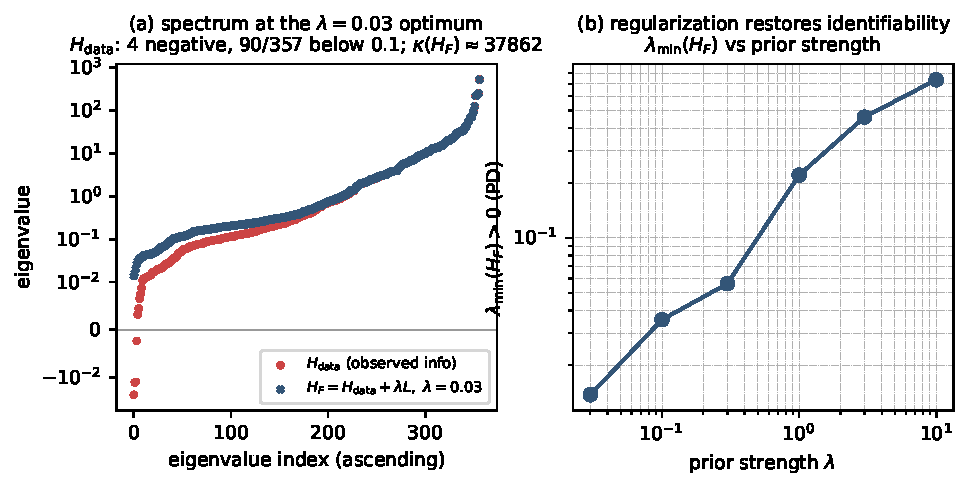
\includegraphics[width=\linewidth]{fig_s53_spectrum.pdf}\\[3pt]
  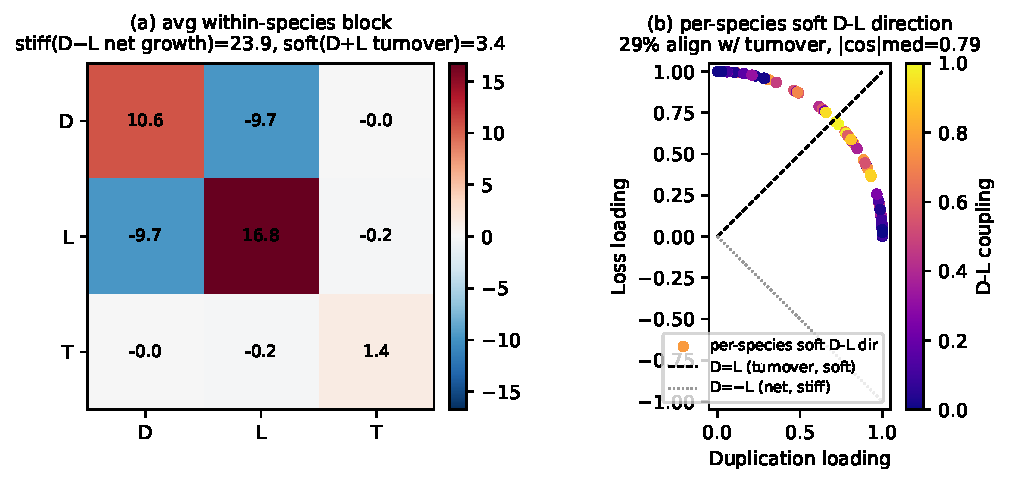
\includegraphics[width=\linewidth]{fig_s53_dl_confounding.pdf}
  \caption{Observed-information analysis at an archaeal species-wise optimum
  ($256$ families, fp64-certified; $p=3S=357$, exact dense $\Fish_{\mathrm{obs}}$).
  \textbf{Top:}
  (left) the data Hessian $\Fish_{\mathrm{obs}}=\Hess_{\mathrm{data}}$ is
  \emph{indefinite} --- $4$ negative eigenvalues and $90/357$ ($25\%$) below
  $0.1$ --- so a quarter of directions are unconstrained by the data alone; the
  GBM prior $\kappa L$ lifts them to make $\Hess_F=\Hess_{\mathrm{data}}+\kappa L$
  positive definite. (right) $\lambda_{\min}(\Hess_F)$ climbs monotonically with
  prior strength ($0.014\!\to\!0.74$ over $\kappa=0.03\!\to\!10$): regularization
  restores identifiability. \textbf{Bottom:} (left) the average within-species
  $3\times3$ block diagonalizes to a \emph{stiff} net-growth axis $\bdelta-\blambda$
  (eig $23.9$) and a \emph{soft} turnover axis $\bdelta+\blambda$ (eig $3.4$);
  transfer is decoupled. (right) per species, the soft duplication--loss direction
  (coloured by D--L coupling) clusters on the turnover diagonal $\bdelta=\blambda$
  --- strongly-coupled species sit exactly on it.}
  \label{fig:fisher}
\end{figure}

\begin{figure}[t]\centering
  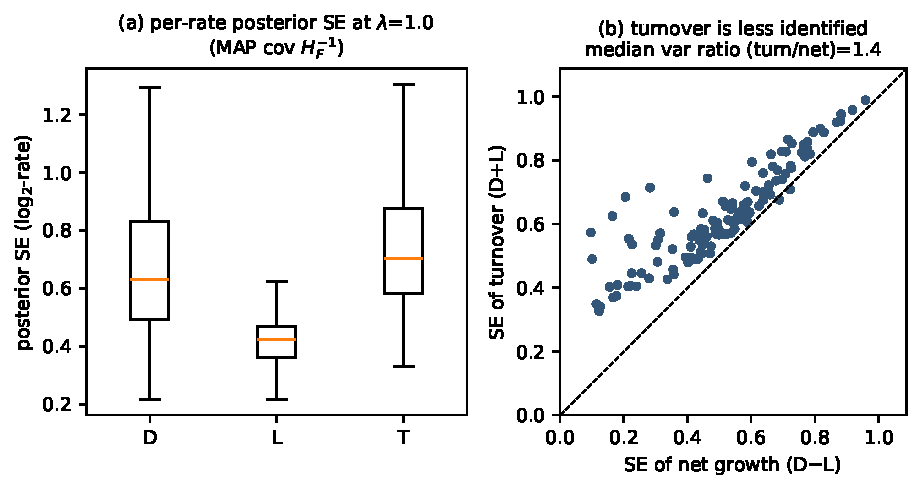
\includegraphics[width=\linewidth]{fig_s53_se.pdf}
  \caption{Laplace (penalized-Hessian/MAP) covariance $\Hess_F^{-1}$ at $\kappa{=}1$ ---
  the lightest tree-smoothing penalty for which $\Hess_F=\Hess_{\mathrm{data}}+\kappa L\succ0$,
  so that the inverse exists; the cross-validated $\kappa^\star{=}0.03$ (Sec.~\ref{sec:cv}) is
  lighter and leaves $\Hess_F$ indefinite. These are MAP credible intervals under the smoothing
  prior, not raw observed-information errors. (left) per-rate posterior standard
  errors (log$_2$-rate): median $\bdelta\!=\!0.63$, $\blambda\!=\!0.42$,
  $\btau\!=\!0.70$ ($95\%$ CI factors $\times/\,2.35,\,1.78,\,2.60$). Transfer,
  though decoupled, carries the \emph{largest} SE --- it is identifiable but only
  gently determined. (right) the turnover combination $\bdelta+\blambda$ has
  $1.4\times$ the posterior variance of net growth $\bdelta-\blambda$ for
  \emph{every} species: turnover is the least-identified direction even after
  regularization.}
  \label{fig:fisher-se}
\end{figure}

\begin{figure}[t]\centering
  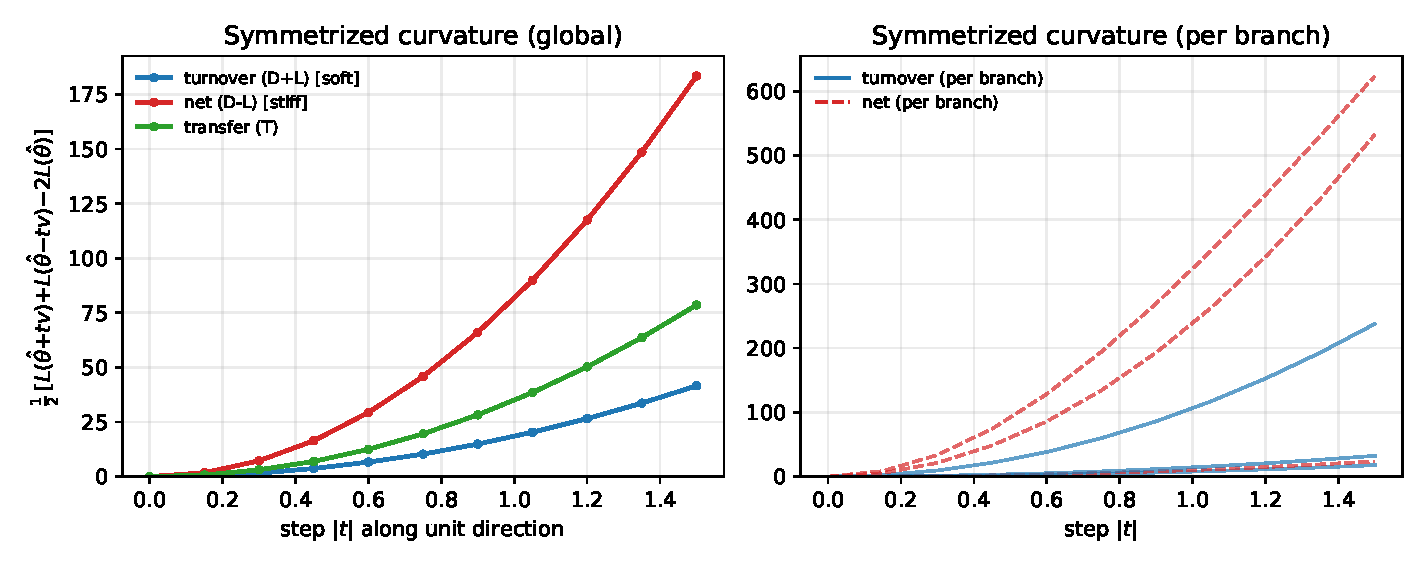
\includegraphics[width=\linewidth]{fig_profile.pdf}
  \caption{Likelihood curvature confirms the eigenvalue geometry. We plot the
  \emph{symmetrized second difference}
  $\tfrac12[L(\hat\theta{+}t v)+L(\hat\theta{-}t v)-2L(\hat\theta)]$ of the data loss
  along unit-normalized rate directions at the certified archaeal fit, summed over all
  $119$ branches (left) and for individual branches (right). Symmetrizing removes the
  first-order term, isolating the local curvature to second order ($\tfrac12 t^2\,v^\top
  \Hess v + O(t^4)$) even though the constrained/penalized fit is not the unconstrained
  data optimum; the plotted quantity is positive wherever the curvature is, and would turn
  negative along a genuinely anti-curved direction. The
  \emph{turnover} axis ($\bdelta{+}\blambda$) is nearly flat (soft), the
  \emph{net-growth} axis ($\bdelta{-}\blambda$) is sharply curved (stiff,
  $\sim\!4\times$ the turnover curvature at $|t|{=}1.5$), and transfer is decoupled and
  intermediate --- the same ordering as the observed-information spectrum
  (Fig.~\ref{fig:fisher}).}
  \label{fig:profile}
\end{figure}

% ----------------------------------------------------------
\subsection{Transfer heterogeneity via per-recipient weights}
\label{sec:receiver}
\paragraph{What is built.} The joint $(\theta,\alpha)$ optimization of
Sec.~\ref{sec:rweights} is fully implemented: the exact gradient
$\partial\NLL/\partial\alpha$, the joint $(\theta,\alpha)$ Hessian--vector product,
and the gauge-projected Fisher information all come from the same analytic backward
as the rates, and each is validated against \texttt{fp64} finite differences to a
per-block relative error of $\sim\!10^{-6}$. A joint box-constrained Newton--CG
optimizer, a deflated-gauge positive-definiteness certificate, and the
gauge-projected receiver Fisher information all come from the same machinery, so
the learned weights carry standard errors and an identifiability diagnosis at no
extra derivation cost.

\paragraph{Full-archaea fit.} Warm-started from the certified rate-only minimum
(Sec.~\ref{sec:certify}; identical box $[0.05,2.0]$ and penalty $\kappa{=}0.03$),
the joint $(\theta,\alpha)$ optimizer was run on all $5{,}446$ families with
box-constrained Newton--CG. The fit is converged to a few nats (final projected
gradient $|P\grad|{=}6.4$, still slowly descending, so the figures below are
conservative \emph{lower bounds}). Relative to the rate-only model with uniform
recipients (data NLL $359{,}561$), the $S{-}1{=}118$ per-branch weights lower the
data NLL to $352{,}494$: a likelihood-ratio improvement of $\approx\!7{,}070$ nats,
about $1.3$ nats per family. Against the cost of the added parameters this is
decisive: $\mathrm{AIC}_{\mathrm{uniform}}-\mathrm{AIC}_{\mathrm{weighted}}\approx
13{,}900$ and $\mathrm{BIC}_{\mathrm{uniform}}-\mathrm{BIC}_{\mathrm{weighted}}\approx
13{,}100$ (both positive, i.e.\ favouring the weighted model; $\approx\!60\times$ the
AIC threshold and $\approx\!14\times$ the BIC threshold). An independent forward-only likelihood
evaluator reproduces the joint optimizer's NLL to $<\!0.1$ nat, ruling out an
optimizer artefact. The inferred recipients are strongly \emph{heterogeneous}: a
handful of branches act as transfer \emph{sinks}, receiving $5$--$8\times$ the
uniform share, while $6$ of $119$ sit at the weight floor (they receive
essentially no transfers). These weights are \emph{tightly determined}, not noisy:
per-recipient standard errors --- the receiver block of the inverse of the exact
free-subspace joint Hessian, marginalized over the $188$ free rates (Schur complement
over the $307$-dimensional free subspace, gauge-projected, two normalization nulls
deflated) --- place every visible sink at $8$--$29$ standard errors above the uniform
share, with $27$ of $119$ branches significantly above uniform. These rate-\emph{marginal}
errors are only modestly larger than the rate-\emph{conditional} ones (median
$1.12\times$, at most $2.8\times$): transfer is largely decoupled from the rates
(Sec.~\ref{sec:fisher}), so accounting for rate uncertainty leaves every qualitative
conclusion intact. Conditional on the model and inputs, then,
the uniform-recipient assumption is decisively rejected and the fitted deviations
nominate recipient-biased archaeal branches --- a statistical claim of recipient
heterogeneity, not yet a claim that these are biologically validated transfer sinks.

\paragraph{Curvature and stability at the joint fit.} We are deliberate
about what the curvature shows. The joint fit reaches $|P\grad|{=}6.4$ and is still
slowly descending, so it is \emph{not} a stationary point and we do not call it an
optimum. The transfer estimate is nonetheless \emph{stable}: a further round of
box-constrained optimization from the reported point lowered the data NLL by only
${\approx}9$ nats and left the recipient weights essentially unchanged (Spearman rank
correlation $0.999$, maximum per-branch change $<\!10^{-3}$), preserving all $10$ of the
top-ranked sinks. The residual gradient therefore lies in flat \emph{rate} directions,
not in the recipient weights on which the model-selection verdict and the standard
errors rest. We also characterize the curvature exactly: the $307$-dimensional
free-subspace joint Hessian ($169$ of $357$ rates box-pinned), formed densely for the
marginal standard errors above, has \emph{no} negative eigenvalue beyond its two gauge
nulls under a \texttt{fp32} dense eigendecomposition (the smallest non-gauge eigenvalue
is positive); a deflated-gauge Lanczos pass ($m{=}200$) agrees, detecting no negative
curvature. The fit therefore sits at a positive-semidefinite, near-flat point --- not a
saddle. This is \emph{not} a strict positive-definiteness certificate: the bottom of the
spectrum clusters at $\approx\!0$ (the weak-identifiability signature of the rates,
Sec.~\ref{sec:certify}) and the point is not tightly converged. A strict \texttt{fp64}
certificate at a tightly-converged optimum is deferred (fp64 Hessian--vector products are
$\sim\!27\times$ slower on the \textsc{RTX 4090}); the model-selection verdict and the
standard errors do not depend on it.

\paragraph{The weights are not a genome-size artifact.} A natural worry is that the
weights merely track \emph{exposure} --- a larger genome receiving more transfers by
opportunity rather than by biology. We test the most obvious such confound, genome size
(gene content, the number of families in which each genome is present). Genome size does
correlate with the recipient weight (Spearman $0.41$, $p{=}10^{-3}$, over the $60$ extant
branches), confirming exposure plays a role; but it explains only ${\approx}20\%$ of the
weight variation ($R^2{=}0.20$ in a log--log fit), and the genome-size-explained recipient
distribution, evaluated at the fitted rates, captures only $44\%$ of the weighted model's
data-NLL gain over uniform recipients ($5{,}562$ of $12{,}639$ nats;
Table~\ref{tab:exposure}). The majority is a residual recipient effect: controlling for
genome size, $8$ of the top $10$ sinks remain top-ranked, and several top sinks are
\emph{small} genomes (e.g.\ \emph{Macid} at the $28$th genome-size percentile,
\emph{CrenYNPFFA} at the $52$nd). The recipient heterogeneity is therefore not a
gene-content/ascertainment artifact. (This is an in-sample sensitivity diagnostic at the
fitted rates; the re-optimized, held-out version is Table~\ref{tab:exposure-cv} below.)

\begin{table}[h]\centering
\caption{Genome size is a real but minority driver of the recipient weights. Data NLL at
the fitted archaeal rates under three recipient distributions (lower is better); the
genome-size-explained distribution replaces each of the $60$ extant leaf lineages' $\log w_s$
by its log--log regression prediction on genome size, leaving the ancestral lineages at their
fitted values. Genome size captures $44\%$ of the gain; $56\%$ is residual recipient effect.
This is a conditional decomposition at fixed weighted-model rates --- not a refit or a
held-out model comparison.}
\label{tab:exposure}
\small
\begin{tabular}{lrr}
\toprule
Recipient distribution (at fitted rates) & data NLL & gain vs.\ uniform \\
\midrule
Uniform                          & $365{,}133$          & --- \\
Genome-size-explained            & $359{,}571$          & $5{,}562$ \;($44\%$) \\
Free recipient weights           & $\mathbf{352{,}494}$ & $\mathbf{12{,}639}$ \;($100\%$) \\
\bottomrule
\end{tabular}
\end{table}

\paragraph{The control survives re-fitting, out of sample.} Table~\ref{tab:exposure} fixes
the rates; a reviewer may still ask whether the recipient effect survives \emph{re-optimization}
under an exposure control. We therefore re-fit each recipient model from scratch on $80\%$ of
families and score the held-out $20\%$, over three random splits (box $[0.05,2.0]$,
$\kappa{=}0.03$; Table~\ref{tab:exposure-cv}). The one-parameter genome-size offset --- recipient
logits $\gamma\log(\text{genome size})$ with $\gamma$ maximum-likelihood-fit per fold --- lowers
the held-out NLL by only $195\pm21$ nats, whereas the free $118$-weight model lowers it by
$1{,}454\pm59$ nats ($1.3$ per held-out family, matching the in-sample gain). Genome size thus
captures $13\%$ of the free model's held-out improvement; the free residual generalizes a further
$1{,}259\pm41$ nats \emph{beyond} exposure, and the top-ten sinks are $9/10$ stable against the
full-data ranking in every split. The recipient heterogeneity is a genuine out-of-sample signal,
not a re-expression of genome size. (The free joint fits on the train folds are box-constrained
descent points, not certified minima --- the joint surface is saddle-prone on subsets --- so the
free held-out advantage is a \emph{conservative} lower bound.)

\begin{table}[h]\centering
\caption{Cross-validated exposure sensitivity. Each recipient model is \emph{re-optimized} on
$80\%$ of the $5{,}446$ families and scored on the held-out $20\%$; entries are the mean over three
random splits (box $[0.05,2.0]$). Unlike Table~\ref{tab:exposure} (a fixed-rate decomposition),
every row here is a held-out, re-fit comparison. The genome-size offset is the one-parameter model
with recipient logits $\gamma\log(\text{genome size})$ on the $60$ extant leaves ($\gamma$ ML-fit per
fold; ancestral lineages at the uniform baseline). The absolute held-out NLL varies by $\sim\!1{,}200$
with fold composition, so the (paired) $\Delta$ vs uniform is the stable quantity. Genome size captures
$13\%$ of the free model's held-out gain; the free residual generalizes $1{,}259\pm41$ nats beyond it.}
\label{tab:exposure-cv}
\small
\begin{tabular}{lrrc}
\toprule
Archaeal model (held-out, re-fit) & held-out NLL & $\Delta$ vs uniform & top-10 overlap \\
\midrule
Uniform recipients              & $74{,}741$          & ---                      & --- \\
Genome-size offset ($1$ dof)    & $74{,}546$          & $-195\pm21$              & --- \\
Free recipient weights ($118$)  & $\mathbf{73{,}287}$ & $\mathbf{-1{,}454\pm59}$ & $9/10$ \\
\bottomrule
\end{tabular}
\end{table}

% ----------------------------------------------------------
\subsection{Held-out validation confirms transfer-recipient heterogeneity}
\label{sec:ablation}
\noindent The $\Delta$AIC of Sec.~\ref{sec:receiver} is in-sample. We validate the
transfer-weight extension \emph{out of sample}, on archaea, where the claim is made
and the parameter/data ratio is defensible ($118$ recipient weights over $5{,}446$
families). A single $80/20$ family split (box $[0.05,2.0]$) fits each model on the
$4{,}356$-family train set and scores data NLL on the $1{,}090$-family held-out set;
the $2\times2$ ablation over \{tree-smoothing\}$\times$\{recipient weights\} is
Table~\ref{tab:ablation}. Adding recipient weights lowers the held-out NLL by
$\approx\!1{,}360$ nats ($1.25$ per held-out family) --- almost exactly the in-sample
gain ($1.30$ per family), so the heterogeneity \emph{generalizes} rather than
overfitting. Tree-smoothing barely moves the held-out likelihood here, because the
box already regularizes the rates; on \textsc{Hogenom}, where no box is used,
smoothing does help held-out ($-88$ NLL, Sec.~\ref{sec:cv}). (The corresponding
free-weight held-out CV on \textsc{Hogenom} is a cluster-scale computation ---
$S{=}1{,}331$ branches, $1{,}330$ weights over $\approx\!844$ train families per
fold, saddle-prone --- and is left to the cluster; archaea is where the
transfer claim is validated.)

\begin{table}[t]\centering
\caption{Held-out transfer-weight ablation (lower NLL is better) on a single
$80/20$ archaeal family split: fit on $4{,}356$ families, score on the $1{,}090$
held-out. Recipient weights cut held-out NLL by $\approx\!1{,}360$ nats; smoothing
adds little (the box regularizes the rates).}
\label{tab:ablation}
\begin{tabular}{lcc}
\toprule
Archaeal model (held-out $20\%$) & Held-out NLL & $\Delta$ vs.\ uniform \\
\midrule
Uniform recipients                & $71{,}619$            & --- \\
\;+ tree-smoothing                 & $71{,}619$            & $\approx 0$ \\
\;+ recipient weights              & $70{,}267$            & $-1{,}352$ \\
\;+ smoothing $+$ recipient weights & $\mathbf{70{,}255}$  & $\mathbf{-1{,}364}$ \\
\bottomrule
\end{tabular}
\end{table}

% ----------------------------------------------------------
\subsection{Tree-smoothing prior: GPU-enabled cross-validation on \textsc{Hogenom}}
\label{sec:cv}
This is the model-selection workflow that GPU throughput makes practical: a
cross-validated choice of penalty strength requires $\#\kappa\times K$ full
species-wise fits, which would be prohibitive on the CPU.

\paragraph{Cross-validation selects a regularizing prior.} On $1{,}055$
\textsc{Hogenom} families with $K{=}5$-fold cross-validation over a grid of
$\kappa$, the tree-smoothing prior of Eq.~\eqref{eq:gbm} improves held-out
likelihood over the unpenalized MLE and selects an \emph{interior} optimum
$\kappa^\star{=}0.03$ (Fig.~\ref{fig:cv}): the mean held-out NLL drops from
$107{,}044$ at $\kappa{=}0$ (the MLE) to $106{,}956$ at $\kappa^\star$
($-88$ over the $\approx\!211$-family held-out fold), while heavy smoothing
over-regularizes ($116{,}137$ at $\kappa{=}1000$). The selected penalty is
\emph{light}: it pulls species-wise rates off the box boundary only partially
(the boundary-saturated fraction falls from $0.43$ at $\kappa{=}0$ to $0.39$ at
$\kappa^\star$, reaching $0.21$ only at the over-smoothed $\kappa{=}1$), so on
\textsc{Hogenom} cross-validation favours mild shrinkage rather than the stronger
penalty that would itself remove the boundary runaway (Sec.~\ref{sec:certify}).
The entire sweep ($\#\kappa\times K$ full fits) runs end-to-end on a single GPU,
which is what makes the protocol practical.

\begin{figure}[t]\centering
  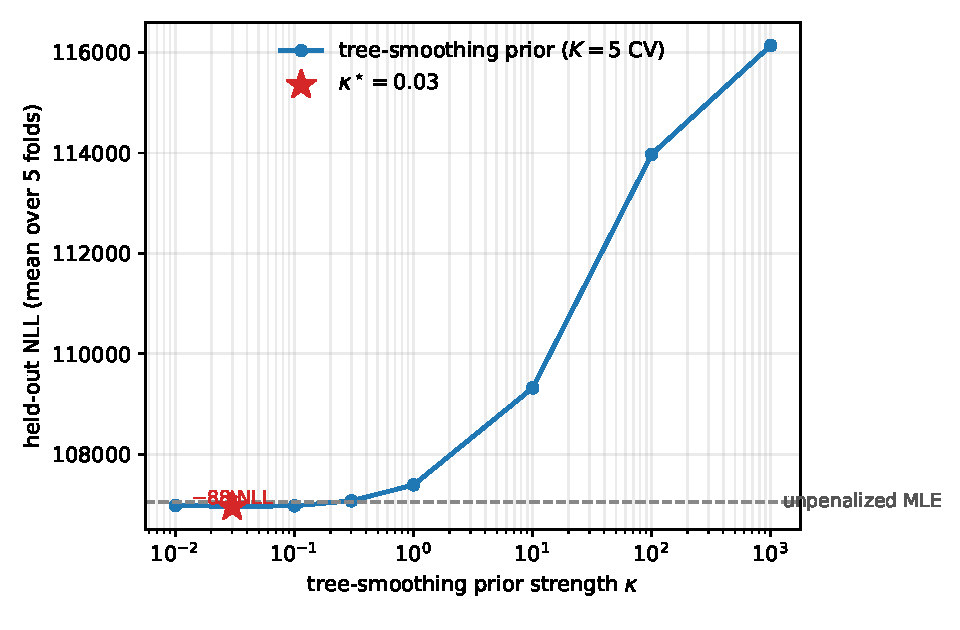
\includegraphics[width=0.62\linewidth]{fig_cv.pdf}
  \caption{Cross-validated selection of the tree-smoothing penalty on $1{,}055$
  \textsc{Hogenom} families (species-wise rates, $K{=}5$ folds). Mean held-out NLL
  vs.\ prior strength $\kappa$ (log scale); the interior optimum is
  $\kappa^\star{=}0.03$, $88$ NLL below the unpenalized MLE (dashed). Heavy
  smoothing ($\kappa\!\gtrsim\!1$) over-regularizes.}
  \label{fig:cv}
\end{figure}

\subsection{Performance: genewise rate estimation an order of magnitude faster}
\label{sec:speed}
Fitting independent per-family DTL rates is the task \textsc{AleRax} performs by
CPU gradient descent. On the \emph{identical} filtered \textsc{Hogenom} set,
\toolname matches its likelihood while running an order of magnitude faster
(Table~\ref{tab:speed-headline}); the per-scale throughput is in
Table~\ref{tab:speed}.

\paragraph{The quality margin is a genuine lower optimum.} Table~\ref{tab:speed-headline}
compares each tool's self-reported NLL. To confirm the difference is a genuinely better
optimum on a single objective rather than an artifact of differing likelihood
evaluations, we re-evaluated \textsc{AleRax}'s fitted rates under \toolname's converged
likelihood ($\pi{=}64$/Neumann${=}64$): \toolname's optimum stays lower, by
$0.22$~nat/family ($2{,}393$~nats over the $10{,}869$ families), and the per-family
difference is zero at the median --- it is concentrated in a minority tail where
\textsc{AleRax}'s reported likelihood falls slightly below the converged re-evaluation
(which accounts for the remaining $\approx\!0.2$~nat/family of the self-reported margin).
The independent same-likelihood cross-check (Table~\ref{tab:validation}, $<\!10^{-3}$ nat
at fixed rates) confirms the two implementations evaluate the same \textsc{UndatedDTL}
likelihood; the speed advantage is therefore obtained at an equal-or-better optimum, not
on a different objective.

\begin{table}[h]\centering
\caption{Head-to-head on the \emph{identical} $10{,}869$-family ($\geq\!4$-species)
\textsc{Hogenom} set --- same species tree, gene-tree distributions,
\textsc{UndatedDTL} model, and $\geq\!4$-species filter. \toolname is
$\sim\!23\times$ faster at a marginally \emph{higher} likelihood (lower NLL).
\textsc{AleRax}~v1.4.0 was run in chunks under an $80$\,GB cap --- exact, since
per-family fits are independent (it otherwise exhausts $>\!300$\,GB loading all
evaluators); its NLL is converted from nats ($\div\ln2$).}
\label{tab:speed-headline}
\begin{tabular}{lcc}
\toprule
 & \textsc{AleRax} (24 CPU cores) & \toolname (1 RTX 4090) \\
\midrule
Wall-clock        & $17{,}682$\,s ($\approx\!4.9$\,h) & $758$\,s \\
Total NLL (bits)  & $1{,}913{,}087$                   & $1{,}906{,}464$ \\
\bottomrule
\end{tabular}
\end{table}

\paragraph{\toolname genewise throughput.} Fitting independent per-family DTL
rates to a converged, box-bounded optimum ($|P\grad|<10^{-3}$, $\rho\in[10^{-6},2]$)
on \textsc{Hogenom} runs entirely on a single RTX 4090: the $10{,}869$ families
covering $\geq\!4$ species --- the set \textsc{AleRax}'s \textsc{UndatedDTL} retains,
making the head-to-head apples-to-apples --- in $\approx\!13$ minutes, with
$99.85\%$ certified converged (interior positive-definite or KKT bound-active).
Per-family throughput \emph{rises} with scale --- $4.3\!\to\!14.3$ families/s from
$506$ to $10{,}869$ --- as batching saturates the GPU (Table~\ref{tab:speed},
Fig.~\ref{fig:speed}). This recipe (Adam warm-up $\to$ box-constrained trust-region
Newton on the per-family $3{\times}3$ forward-difference Hessian, with
convergence-based rebatching and $\pi$-tier escalation) is the \toolname library
default, \texttt{gpurec.fit\_genewise}. The adjoint warm-start that makes the cheap
$\pi{=}16$ tier accurate carries a resident cache scaling as
clades${\times}$species${\times}$dtype --- the dominant allocation, $\approx\!19$\,GiB
on the full set; a memory-aware gate keyed on that product runs the large early
batches cold and re-enables the warm-start as the active set shrinks, keeping the
full dataset within the $24$\,GB device with no manual tuning.

\begin{table}[t]\centering
\caption{\toolname genewise rate-fitting throughput on \textsc{Hogenom}, restricted to families
covering $\geq\!4$ species (the set \textsc{AleRax} retains; \#families is after the filter, from
nominal draws of $512$/$1{,}055$/all). Single RTX 4090, library recipe \texttt{gpurec.fit\_genewise}
($|P\grad|<10^{-3}$, $\rho\in[10^{-6},2]$). Wall-clock is the optimize time; the converged count
and total NLL (bits) come from an optional cold PD certificate ($\pi{=}64$/Neumann${=}64$).
Per-family throughput rises with scale ($4.3\!\to\!14.3$ families/s) as batching saturates the GPU.}
\label{tab:speed}
\begin{tabular}{lrrr r}
\toprule
Dataset & \#families & wall-clock & converged & total NLL (bits) \\
\midrule
\textsc{Hogenom}-512   & $506$      & $119$\,s   & $500/506$           & $324{,}262$ \\
\textsc{Hogenom}-1055  & $1{,}042$  & $219$\,s   & $1{,}037/1{,}042$   & $577{,}593$ \\
\textsc{Hogenom}-full  & $10{,}869$ & $758$\,s   & $10{,}853/10{,}869$ & $1{,}906{,}464$ \\
\bottomrule
\end{tabular}
\end{table}

\begin{figure}[t]\centering
  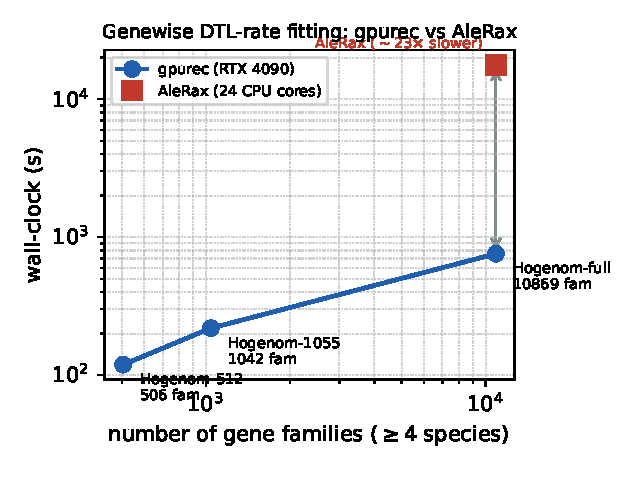
\includegraphics[width=0.62\linewidth]{fig_speed.pdf}
  \caption{Genewise DTL-rate fitting wall-clock vs.\ number of gene families on
  \textsc{Hogenom} (single RTX 4090; log--log). Throughput improves with scale as
  batching saturates the GPU (per-family rate rising from $4.3$ to $14.3$
  families/s). The head-to-head against \textsc{AleRax} on the full
  $10{,}869$-family set is reported in Table~\ref{tab:speed-headline}.}
  \label{fig:speed}
\end{figure}

% ----------------------------------------------------------

% =====================================================================
\section{Discussion}
\label{sec:discussion}

\paragraph{An extensible, differentiable engine.} The unifying theme is that a
single design choice --- implementing the reconciliation likelihood as a
differentiable GPU program --- yields speed, second-order inference, and model
flexibility together. New terms (priors, alternative recipient models,
hierarchical rate structure) are written as \textsc{PyTorch} expressions and
require \emph{no} hand-derived gradients or Hessians; they immediately inherit
the optimizer, the HVP-based certification, and the Fisher-information tooling.

\paragraph{Simplicity and reproducibility.} The model can be constructed and
optimized in a few lines in a Jupyter notebook, with direct programmatic access
to the loss, gradient, Hessian--vector product, and per-batch solver controls.
This lowers the barrier to methodological experimentation and makes analyses
reproducible.

\paragraph{From a tool to a platform.} The same differentiable core that gives
the results above also makes several extensions natural rather than bespoke: a
Laplace approximation to the posterior over rates (Bayesian uncertainty without
MCMC), hierarchical priors in which species-wise rates inherit from clade-level
hyperparameters, and the use of differentiable reconciliation as the inner
objective of a species-tree search. We develop these in
Appendix~\ref{app:outlook}; collectively they reframe \toolname as a platform
for model development rather than a single fixed tool.

\paragraph{Interpreting the recipient weights.} What the held-out likelihood and the
$\Delta$AIC establish is statistical: the uniform-recipient model is decisively
inferior to one in which transfer recipients are non-uniform across branches. That a
particular branch carries a high fitted weight should be read as a \emph{model-conditional
nomination}, not a validated biological transfer sink. A per-branch weight can absorb
non-biological structure --- uneven taxon sampling, genome size and gene-family
ascertainment, donor-opportunity imbalance (a branch contemporaneous with many potential
donors), branch placement and species-tree uncertainty, and systematic gene-tree error
--- any of which can mimic preferential reception. We have already controlled for the most
obvious one, genome size, both in-sample (Sec.~\ref{sec:receiver}, Table~\ref{tab:exposure}:
it accounts for only $\approx\!20\%$ of the weight variation, $8/10$ top sinks survive) and
out-of-sample under re-optimization (Table~\ref{tab:exposure-cv}: a maximum-likelihood
genome-size offset captures only $13\%$ of the free model's held-out gain, the free residual
generalizing $1{,}259$ nats beyond it, with $9/10$ top sinks stable) --- so the effect is not a
gene-content artifact. The remaining controls (sampling density, donor-opportunity imbalance,
branch-placement and species-tree uncertainty, systematic gene-tree error) are each a cheap
re-fit under a perturbed input or an added covariate in the same differentiable framework, the
natural continuation of the held-out exposure analysis already in hand. We therefore present
the archaeal weights as a robust \emph{statistical} rejection of the uniform-recipient
assumption --- one that survives a genome-size control out of sample --- together with a ranked
set of candidate recipient-biased lineages, and defer full biological attribution to that
broader sensitivity analysis.

\paragraph{Limitations.} (i) We address rate estimation and reconciliation
given a fixed species tree and CCP inputs; species-tree search is out of scope
here. (ii) Per-recipient weights and per-species rates add parameters and rely
on the regularization of Sec.~\ref{sec:cv} to remain identifiable. (iii) GPU
memory bounds the largest single batch; we mitigate this with batching and
adaptive solver fidelity. (iv) On the full archaeal data, per-recipient transfer
weights are decisively favoured both in-sample (AIC/BIC) and out-of-sample (held-out
NLL, Sec.~\ref{sec:ablation}), with rate-marginalized per-weight standard errors and a
no-negative-curvature check in hand (Sec.~\ref{sec:receiver}); the in-sample and held-out
evidence already carries the claim. As a small simulation \emph{sanity check} --- not a
pillar of the result --- we probed the non-standard likelihood-ratio regularity under the
box/floor/gauge constraints with a parametric bootstrap: simulating gene families under
the fitted uniform-recipient \textsc{UndatedDTL} model (with an independent simulator we
verified against ours by rate recovery) and refitting both models, the null
likelihood-ratio statistic concentrates tightly at $\Delta\ell\!\approx\!95.5$ nats
($B{=}8$, s.d.\ $0.7$) --- about $1.6\times$ the naive $\chi^2$ value of $59$ (half the
$118$ added weights), so the constraints \emph{do} inflate the null above the standard
asymptotic, yet the observed $\Delta\ell\!\approx\!7{,}070$ sits roughly $70\times$ outside
it. A strict \texttt{fp64} certificate of a tightly-converged joint optimum and a larger
matched-scale bootstrap ($B\!\gtrsim\!200$) are useful extensions, but are not required for
the claims made here.

% =====================================================================
\section{Conclusion}
\label{sec:conclusion}
We presented \toolname, a GPU-accelerated, differentiable implementation of the
\textsc{UndatedDTL} amalgamated reconciliation likelihood. Beyond an
order-of-magnitude speedup for genewise rate estimation, differentiability
gives certified optima, observed-information and penalized-Hessian uncertainty,
identifiability analysis, user-defined penalties with cross-validated model
selection, and learned transfer heterogeneity --- capabilities that are
difficult or impossible with existing CPU, first-order tools, and that follow
naturally from exposing reconciliation through a \textsc{PyTorch} interface.

% =====================================================================
\section*{Availability}
\toolname is implemented as an editable \textsc{PyTorch} package plus a
\textsc{Rust} preprocessing extension (built with \texttt{cargo build --release};
the resulting shared library is located via the \texttt{GPUREC\_PREPROCESS\_PATH}
environment variable). Each completed result here is produced by a
self-contained driver under \texttt{experiments/sanderson\_cv/},
\texttt{experiments/receiver\_robustness/}, or
\texttt{benchmarks/hogenom-cpu-vs-gpu/scripts/}, runnable on one GPU where
required and writing a self-describing artifact:
\begin{itemize}[nosep]
\item \textbf{Speed (Sec.~\ref{sec:speed})} ---
  \texttt{benchmarks/hogenom-cpu-vs-gpu/scripts/reproduce.sh}:
  per-family rates to $|P\grad|<10^{-3}$ on \textsc{Hogenom}.
\item \textbf{Certified optimum (Sec.~\ref{sec:certify})} ---
  \texttt{converge\_bounded\_archaea.py}: the box-constrained free-subspace
  trust-region Newton--CG with negative-curvature escape and the reduced-Hessian
  positive-definiteness certificate.
\item \textbf{Observed information (Sec.~\ref{sec:fisher})} ---
  \texttt{fisher\_information\_s53.py}: the dense $\Fish_{\mathrm{obs}}$ spectrum,
  the duplication--loss confounding, and asymptotic standard errors.
\item \textbf{Cross-validation (Sec.~\ref{sec:cv})} ---
  \texttt{run\_cv.py}: $K$-fold tree-smoothing cross-validation over a $\kappa$ grid.
\item \textbf{Transfer weights + held-out validation (Secs.~\ref{sec:receiver},~\ref{sec:ablation})}
  --- \texttt{converge\_bounded\_joint\_archaea.py} (joint $(\theta,\alpha)$ fit, certificate,
  receiver Fisher), \texttt{archaea\_heldout.py} (the $80/20$ held-out ablation), and
  \texttt{archaea\_exposure\_cv.py} (the cross-validated genome-size exposure-sensitivity table,
  with \texttt{build\_genome\_sizes.py} for the covariate);
  \texttt{profile\_slices.py} for the likelihood-geometry figure (Sec.~\ref{sec:fisher}).
\end{itemize}
\paragraph{Data and code availability.} The empirical inputs are the published
\textsc{Hogenom} \citep{Penel2009} and archaeal \citep{Davin2018} CCP collections; each
driver reads its data root from an environment variable. In line with the journal's
data-availability policy, at submission the datasets (CCP inputs and fitted artifacts, with
input hashes) are deposited in \textsc{Dryad} with a reviewer-accessible URL, and the
source, the \textsc{Rust} preprocessing extension, exact run commands, and
figure-regeneration scripts are deposited in \textsc{Zenodo} with a reviewer-accessible
private link; the public \textsc{Dryad} and \textsc{Zenodo} DOIs are activated on
acceptance.

% =====================================================================
\appendix
\section{Extensions and outlook: differentiable reconciliation as a platform}
\label{app:outlook}
The capabilities in the main text all follow from one design choice --- a
differentiable, GPU-resident reconciliation likelihood with analytic gradients and
Hessian--vector products. The same machinery makes the following extensions
natural; we sketch them here as the roadmap that distinguishes \toolname from a
single fixed tool. None requires hand-derived derivatives: each is expressed as
a \textsc{PyTorch} term and inherits the optimizer, the matrix-free HVP, and the
information-matrix tooling.

\subsection{Bayesian inference by Laplace approximation}
\label{app:laplace}
Because the Hessian at the MAP/ML estimate is available matrix-free, the
posterior over rates admits a Gaussian (Laplace) approximation
\begin{equation}
  p(\theta \mid D) \;\approx\; \mathcal{N}\!\left(\hat\theta,\; \Hess(\hat\theta)^{-1}\right),
  \label{eq:laplace}
\end{equation}
giving credible intervals and posterior correlations \emph{without} MCMC. The
required linear solves with $\Hess$ reuse the same matrix-free conjugate-gradient
/ Lanczos routines used for optimization and certification; one never forms or
inverts the dense Hessian. This turns the point estimates that current
reconciliation tools report into full uncertainty statements, and enables
penalty-based (marginal-likelihood / information-criterion) model comparison
between the extensions of Sec.~\ref{sec:penalty}--\ref{sec:rweights}.

\subsection{Hierarchical (clade-level) rate priors}
\label{app:hier}
The penalty framework of Sec.~\ref{sec:penalty} generalizes to a hierarchy:
per-species rates $\theta_s$ can be drawn from clade-level hyper-parameters
$\mu_c$ (themselves estimated), e.g.\ $\theta_s \sim \mathcal{N}(\mu_{c(s)},
\sigma^2)$ with the tree-Laplacian (Eq.~\eqref{eq:gbm}) as the special case of a
single global level. This partial pooling shares strength among related lineages
--- regularizing the weakly-identified directions diagnosed in
Sec.~\ref{sec:fisher} --- and is again just an additional differentiable term in
$R(\theta)$, with the hyper-parameters optimized (empirical Bayes) or integrated
(via the Laplace approximation of App.~\ref{app:laplace}).

\subsection{Differentiable reconciliation inside species-tree search}
\label{app:treesearch}
The main text fixes the species tree $S$. Species-tree inference
(\textsc{SpeciesRax}/\textsc{AleRax}) searches over $S$ by SPR moves, recomputing
rates at each candidate. A fast, differentiable rate-estimation inner loop is
exactly the expensive primitive that search repeatedly invokes; \toolname can
serve as that inner objective, and the gradient/curvature it exposes opens the
possibility of continuous relaxations of branch-level structure. We leave a full
treatment to future work, but note that the engine presented here is the
component such a search would be built around.

\subsection{Other consequences}
\label{app:other}
The same interface supports: alternative recipient models beyond the softmax of
Sec.~\ref{sec:rweights} (any differentiable parameterization); gradient-based
sensitivity analysis of inferred DTL event counts to the rates; and integration
with the broader differentiable-programming ecosystem (e.g.\ amortized or
variational inference over rates). Each is a direct consequence of exposing the
likelihood, its gradient, and its curvature through a standard autodiff
interface.

% =====================================================================
\begin{thebibliography}{99}
\small

\bibitem[Morel et~al.(2024)]{Morel2024} Morel B, Williams TA, Stamatakis A, Sz\"oll\H{o}si GJ.
AleRax: a tool for gene and species tree co-estimation and reconciliation under
a probabilistic model of gene duplication, transfer, and loss.
\emph{Bioinformatics} 2024;40(4):btae162.

\bibitem[Morel et~al.(2022)]{Morel2022} Morel B, Schade P, Lutteropp S, et al. SpeciesRax: a tool
for maximum likelihood species tree inference from gene family trees under
duplication, transfer, and loss. \emph{Mol Biol Evol} 2022;39:msab365.

\bibitem[Morel et~al.(2020)]{Morel2020} Morel B, Kozlov AM, Stamatakis A, Sz\"oll\H{o}si GJ.
GeneRax: a tool for species-tree-aware maximum likelihood-based gene family tree
inference under gene duplication, transfer, and loss.
\emph{Mol Biol Evol} 2020;37:2763--2774.

\bibitem[Sz\"oll\H{o}si et~al.(2013)]{Szollosi2013} Sz\"oll\H{o}si GJ, Rosikiewicz W, Boussau B, et al.
Efficient exploration of the space of reconciled gene trees.
\emph{Syst Biol} 2013;62:901--912.

\bibitem[Sz\"oll\H{o}si et~al.(2015)]{Szollosi2015} Sz\"oll\H{o}si GJ, Tannier E, Daubin V, Boussau B. The
inference of gene trees with species trees. \emph{Syst Biol} 2015;64:e42--e62.

\bibitem[H\"ohna and Drummond(2012)]{Hohna2012} H\"ohna S, Drummond AJ. Guided tree topology proposals for
Bayesian phylogenetic inference. \emph{Syst Biol} 2012;61:1--11.

\bibitem[Larget(2013)]{Larget2013} Larget B. The estimation of tree posterior probabilities
using conditional clade probability distributions.
\emph{Syst Biol} 2013;62:501--511.

\bibitem[Sanderson(2002)]{Sanderson2002} Sanderson MJ. Estimating absolute rates of molecular
evolution and divergence times: a penalized likelihood approach.
\emph{Mol Biol Evol} 2002;19:101--109.

\bibitem[Penel et~al.(2009)]{Penel2009} Penel S, Arigon A-M, Dufayard J-F, et al. Databases of
homologous gene families for comparative genomics.
\emph{BMC Bioinformatics} 2009;10:S3.

\bibitem[Williams et~al.(2017)]{Williams2017} Williams TA, Sz\"oll\H{o}si GJ, Spang A, et al.
Integrative modeling of gene and genome evolution roots the archaeal tree of
life. \emph{Proc Natl Acad Sci USA} 2017;114:E4602--E4611.

\bibitem[Dav\'in et~al.(2018)]{Davin2018} Dav\'in AA, Tannier E, Williams TA, et al. Gene transfers
can date the tree of life. \emph{Nat Ecol Evol} 2018;2:904--909.

\bibitem[Felsenstein(1988)]{Felsenstein1988} Felsenstein J. Phylogenies from molecular sequences:
inference and reliability. \emph{Annu Rev Genet} 1988;22:521--565.

\bibitem[Zhang and Mirarab(2022)]{Zhang2022} Zhang C, Mirarab S. ASTRAL-Pro 2: ultrafast species tree
reconstruction from multi-copy gene family trees.
\emph{Bioinformatics} 2022;38:4949--4950.

\bibitem[Paszke et~al.(2019)]{Paszke2019} Paszke A, Gross S, Massa F, et al. PyTorch: an imperative
style, high-performance deep learning library. \emph{NeurIPS} 2019.

\bibitem[Kingma and Ba(2015)]{Kingma2015} Kingma DP, Ba J. Adam: a method for stochastic
optimization. \emph{ICLR} 2015.

\bibitem[Liu and Nocedal(1989)]{LiuNocedal1989} Liu DC, Nocedal J. On the limited memory BFGS method
for large scale optimization. \emph{Math Program} 1989;45:503--528.

\bibitem[Lanczos(1950)]{Lanczos1950} Lanczos C. An iteration method for the solution of the
eigenvalue problem of linear differential and integral operators.
\emph{J Res Natl Bur Stand} 1950;45:255--282.

\end{thebibliography}

\end{document}
